%%%%%%%%%%%%%%%%%%%%%%%%%%%%%%%%%%%%%%%%%%%%%%%%%%%%%%%%%%%%%%%%%%%%%%%%%%%%%%%%%%%%%%%%%
% 
% Template for DEE@ISEP Presentations, for LEEC, LETI and MEEC
% developed by Vitor M. R. Cunha - v1.0, Mar 2024
% Suggestions and comments are welcomed (vrc at isep dot ipp dot pt).
%
% Template provided as is, NO SUPPORT will be given.
% NO questions related to Beamer (or LaTeX) will be answered, go to
% https://tug.ctan.org/macros/latex/contrib/beamer/doc/beameruserguide.pdf, or search the web.
%
%%%%%%%%%%%%%%%%%%%%%%%%%%%%%%%%%% CLASS SETTINGS %%%%%%%%%%%%%%%%%%%%%%%%%%%%%%%%%%%%%%

\documentclass[
aspectratio=169,	% Comment for 4:3 aspect ratio
LEEC,				% Use this option to select your DEE degree, options: LEEC, LETI
portuguese,			% Select document language, options: portuguese, english
%handout			% Uncomment to make the PDF WITHOUT overlays, e.g., for PDF submission before the presentation 
]{DEEclassP}
\usepackage{tikz}
\usepackage{amsmath}
\usetikzlibrary{arrows.meta, positioning}
% Use the 'preamble.tex' file (root folder) do add packages and macros. Keep your main.tex file clean.

%%%%%%%%%%%%%%%%%%%%%%%%%%%%%%%%%%%%%%%%%%%%%%%%%%%%%%%%%% packages
\usepackage{amsmath}		% the main package in the AMS-LATEX distribution
\usepackage{amsfonts}		% extended set of fonts for use in mathematics
\usepackage{amssymb}		% adds new symbols to be used in math mode
\usepackage{mathrsfs}		% math fonts, e.g., Laplace	
\usepackage{float}			% provides the H float modifier option
\usepackage{multirow}		% tables \multirow command
\usepackage{subcaption}		% enables subfigures					 
\usepackage{siunitx}
\usepackage{textcomp}
\usepackage{gensymb}		% typesetting of units				
\usepackage{verbatim}		% new verbatim environment, \begin{comment}...\end{comment}, \verbatiminput	
\usepackage[main=russian,english]{babel}
\usepackage{wrapfig}
\usepackage{multicol}
\usepackage{graphicx} % Пакеты для вставки графики
\usepackage{subfig}
\usepackage[flushleft]{threeparttable}
\usepackage{bm}
\usepackage{algorithm}
\usepackage{algpseudocode}
\usepackage[backend=biber,style=verbose-note]{biblatex}
\bibliography{sampleRefs}  % Link your bibliography file
\usepackage{booktabs} % for better looking tables
\usepackage{adjustbox} % for adjusting table to fit within slide
\usepackage[table]{xcolor} % for coloring cells
% Define a custom color (light blue) for the header
\definecolor{headerblue}{RGB}{208,227,242}
%add extra packages if needed here

%%%%%%%%%%%%%%%%%%%%%%%%%%%%%%%%%%%%%%%%%%%%%%%%%%%%%%%%%% settings


%%%%%%%%%%%%%%%%%%%%%%%%%%%%%%%%%%%%%%%%%%%%%%%%%%%%%%%%%% user macros
\newcommand{\cc}[1]{\mathcal{#1}}
\newcommand{\bb}[1]{\mathbb{#1}}
\newcommand{\bR}{\mathbb{R}}
\newcommand{\bE}{\mathbb{E}}
\newcommand{\x}{\bm{x}}
\newcommand{\z}{\bm{z}}



\AtBeginSection[]{
  \begin{frame}
  \vfill
  \centering
  \begin{beamercolorbox}[sep=8pt,center,shadow=true,rounded=true]{title}
    \usebeamerfont{title}\insertsectionhead\par%
  \end{beamercolorbox}
  \vfill
  \end{frame}
}

%%%%%%%%%%%%%%%%%%%%%%%%%%%%% PRESENTATION INFORMATION %%%%%%%%%%%%%%%%%%%%%%%%%%%%%%%%%%

\title{Численное решение модели реального делового цикла для закрытой экономики}
\author{Козлов Кирилл Андреевич}
% \author[]{Аветисян Арам Арутюнович}
% \author[Маркин Юрий Витальевич]{}
\predate{\today} 					% Presentation date, comment this line for automatic date (today)

%%%%%%%%%%%%%%%%%%%%%%%%%%%%%%%%%%%%%%%%%%%%%%%%%%%%%%%%%%%%%%%%%%%%%%%%%%%%%%%%%%%%%%%%%
\begin{document}

\begin{frame}[noframenumbering,plain]
	\titlepage
\end{frame}

% \begin{frame}{Структура}
% 	\tableofcontents
% \end{frame}
%%%%%%%%%%%%%%%%%%%%%%%%%%%%%% MAKE YOUR SLIDES AFTER THIS %%%%%%%%%%%%%%%%%%%%%%%%%%%%%%



\begin{frame}{Актуальность задачи}
\small
\begin{minipage}[t]{0.72\textwidth}
\begin{itemize}
    \item Центральные банки по всему миру, включая Банк России, используют DSGE-модели для макроэкономического прогнозирования и анализа последствий денежно-кредитной политики, рассматривая их как часть своего ключевого аналитического аппарата.
    \item В свою очередь, инвестиционные фонды применяют аналогичные RBC/DSGE-модели для количественной оценки влияния макроэкономических шоков, например, изменений производительности, на доходность активов и обоснования своих инвестиционных стратегий.
\end{itemize}
\end{minipage}
\hfill
\begin{minipage}[t]{0.24\textwidth}
    \centering
    
\includegraphics[width=\linewidth]{theme/cb.png}
\end{minipage}
\end{frame}

%%%%%%%%%%%%%%%%%%%%%%%%%%%%%%%%%%%%%%%%%%%%%%%%%%%%%%%%%%%%%%%%%%%%%%%%%%%%%%%%%%%%%%%%%
\begin{frame}{Постановка задачи}
\small
\begin{itemize}
    \item Требуется численно исследовать модель реального делового цикла для закрытой экономики в двух постановках --- детерминированной и стохастической.
    \item Для детерминированной версии задача решается аналитическим нахождением стационарного состояния и численным решением с помощью метода стрельбы, а для стохастической версии анализируется стационарное состояние, импульсные отклики и влияние технологических и монетарных шоков на основные макроэкономические переменные.
\end{itemize}
\end{frame}

\begin{frame}{Описание модели}
\scriptsize

\begin{itemize}
    \item Агенты: репрезентативное домохозяйство, репрезентативная фирма.
    \item Домохозяйство (максимизация полезности):
\end{itemize}
\[
\max_{\{C_t,L_t,K_{t+1}\}_{t=0}^{\infty}}
\sum_{t=0}^{\infty}\beta^t
\left(
\frac{C_t^{1-\sigma}}{1-\sigma}
-\phi\frac{L_t^{1+\psi}}{1+\psi}
\right)
\]
\[
C_t+K_{t+1}=w_tL_t+R_tK_t+(1-\delta)K_t.
\]

\begin{itemize}
    \item Фирма (производство): \(Y_t=AK_t^{\alpha}L_t^{1-\alpha}\).
    \item Условия первого порядка (FOC):
\end{itemize}
\begin{align*}
C_t^{-\sigma} &= \beta C_{t+1}^{-\sigma}(R_{t+1}+1-\delta)
&& \text{(уравнение Эйлера)},\\
\phi L_t^{\psi} &= w_t C_t^{-\sigma}
&& \text{(выбор труда)},\\
R_t &= \alpha\frac{Y_t}{K_t},\quad
w_t=(1-\alpha)\frac{Y_t}{L_t}
&& \text{(предельные продукты)}.
\end{align*}
\end{frame}

\begin{frame}{Описание модели}
\scriptsize
\textbf{Для решения модели необходимо найти стационарное состояние (SS)}

\begin{itemize}
    \item Стационарное состояние (SS):
    \(K_t=K^*,\ C_t=C^*,\ L_t=L^*\).
\end{itemize}
\begin{align*}
1 &= \beta\left(\alpha A (K^*)^{\alpha-1}(L^*)^{1-\alpha}+1-\delta\right),\\
\alpha A\left(\frac{K^*}{L^*}\right)^{\alpha-1} &= \frac{1}{\beta}-1+\delta,\\
C^* &= A(K^*)^{\alpha}(L^*)^{1-\alpha}-\delta K^*,\\
\phi(L^*)^{\psi} &= (1-\alpha)A\left(\frac{K^*}{L^*}\right)^{\alpha}(C^*)^{-\sigma}.
\end{align*}

\begin{itemize}
    \item Численное решение: лог-линеаризация системы FOC; метод стрельбы для подбора начального потребления \(C_0\); построение фазовых портретов и временных рядов.
    \item Параметры: \(\beta=0.96,\ \alpha=0.33,\ \delta=0.1,\ \sigma=1,\ \phi=0.75,\ \psi=0.35\).
\end{itemize}
\end{frame}



%%%%%%%%%%%%%%%%%%%%%%%%%%%%%%

%%%%%%%%%%%%%%%%%%%%%%%%%%%%%%

\begin{frame}{Обзор решений: Локальные методы решения RBC}
\scriptsize
\textbf{Метод пертурбаций (возмущений).}
Локальный подход: условия модели разлагаются в ряд Тейлора в окрестности детерминированного стационарного состояния (SS).
Решение получается аналитическим (в виде полиномов) и вычисляется очень быстро, но остается точным только в малой окрестности SS.

\vspace{0.25em}
\begin{itemize}
    \item Исходная задача аппроксимируется рядом Тейлора, после чего строятся локальные правила управления.
    \item При больших шоках и высокой волатильности точность заметно падает; для глобальной динамики метод ограничен.
    \item \textbf{Бланшар-Кан (1980):} для линеаризованных RE-моделей; детерминированность есть, когда число корней вне единичного круга равно числу ``прыгающих'' переменных.
    \item \textbf{Симс (2002):} более общий матричный подход (QZ-разложение), включая случаи с сингулярными матрицами.
    \item \textbf{Результат (Determinacy):} единственное решение существует только при седловой устойчивости (saddle-path stable).
\end{itemize}
\end{frame}

\begin{frame}{Обзор решений: Глобальные методы решения RBC}
\scriptsize
В отличие от локальных, глобальные методы не линеаризуют модель и ищут численное решение на всем пространстве состояний. Это важно для больших шоков, нелинейностей и ограничений.

\vspace{0.25em}
\begin{itemize}
    \item \textbf{Метод Стрельбы (shooting):} подбор начального \(C_0\), чтобы траектория по уравнению Эйлера пришла в SS; в вашей реализации используется бисекция с сужением интервала по направлению движения \(K\) и \(C\).
    \item \textbf{Метод проекций (Projection / Weighted Residuals):} решение аппроксимируется, например, полиномами Чебышева; коэффициенты выбираются так, чтобы минимизировать невязку во всей области. Обычно точнее пертурбаций для нелинейных моделей.
    \item \textbf{Итерация по функции ценности (VFI):} итеративное решение уравнения Беллмана для \(V(K)\); естественно учитывает ограничения типа \(K_{t+1}\ge 0\) и сложные нелинейности.
\end{itemize}
\end{frame}

\begin{frame}{Численное решение RBC: фазовые траектории}
\centering
\begin{minipage}{0.49\textwidth}
    \centering
    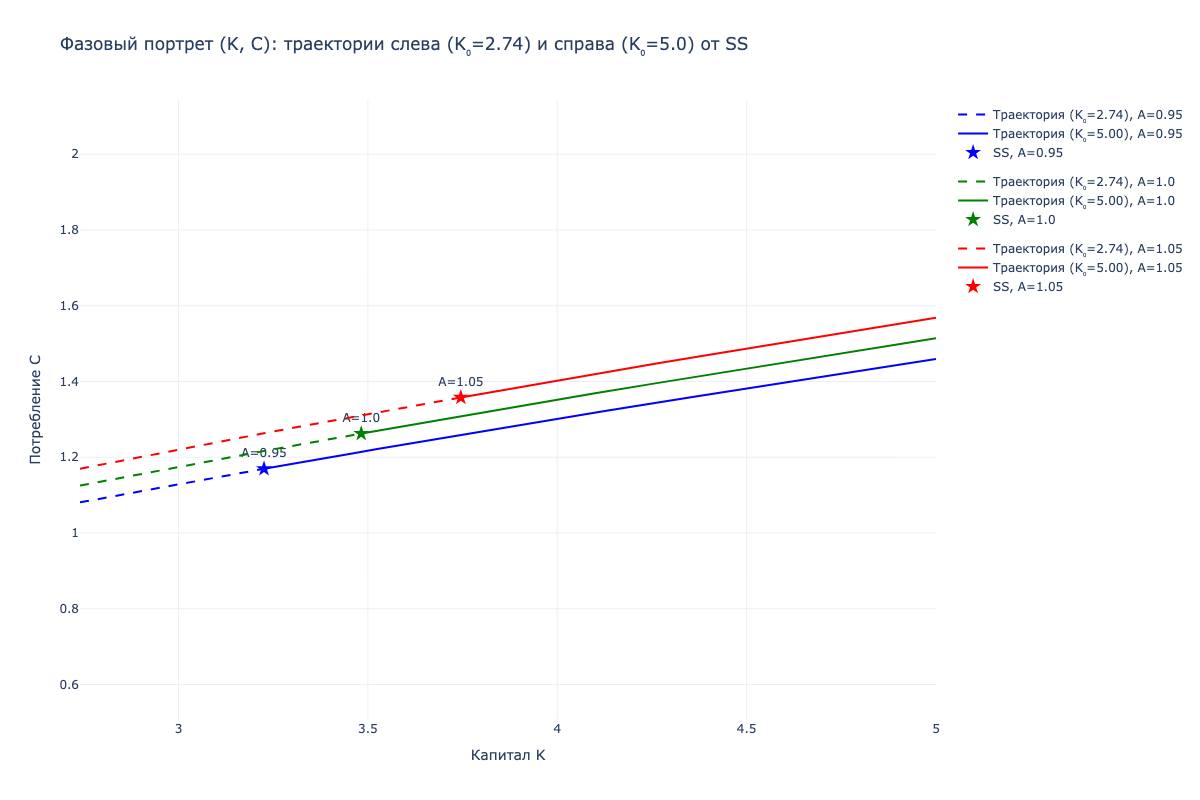
\includegraphics[width=\linewidth,height=0.68\textheight,keepaspectratio]{plots/rbc_solution_kc.png}
\end{minipage}
\hfill
\begin{minipage}{0.49\textwidth}
    \centering
    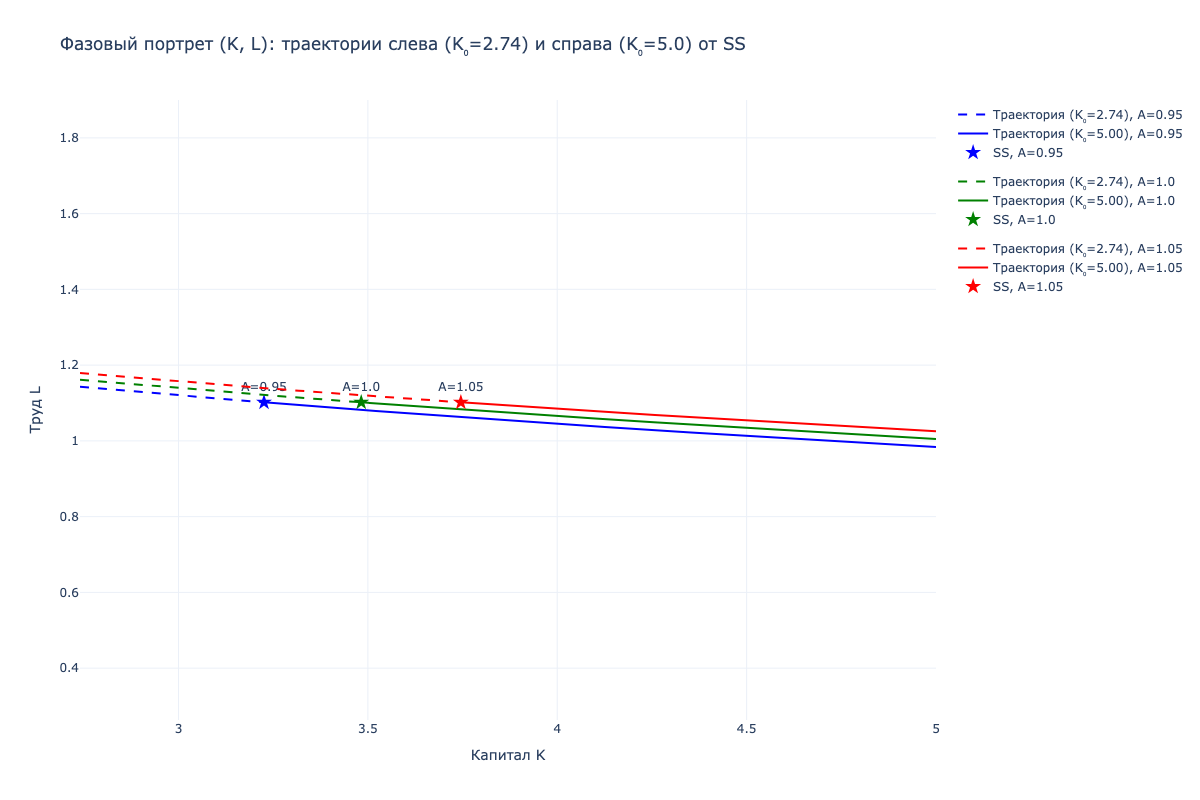
\includegraphics[width=\linewidth,height=0.68\textheight,keepaspectratio]{plots/rbc_solution_kl.png}
\end{minipage}
\end{frame}

\begin{frame}{Численное решение RBC: 3D траектория}
\centering
\begin{minipage}{0.49\textwidth}
    \centering
    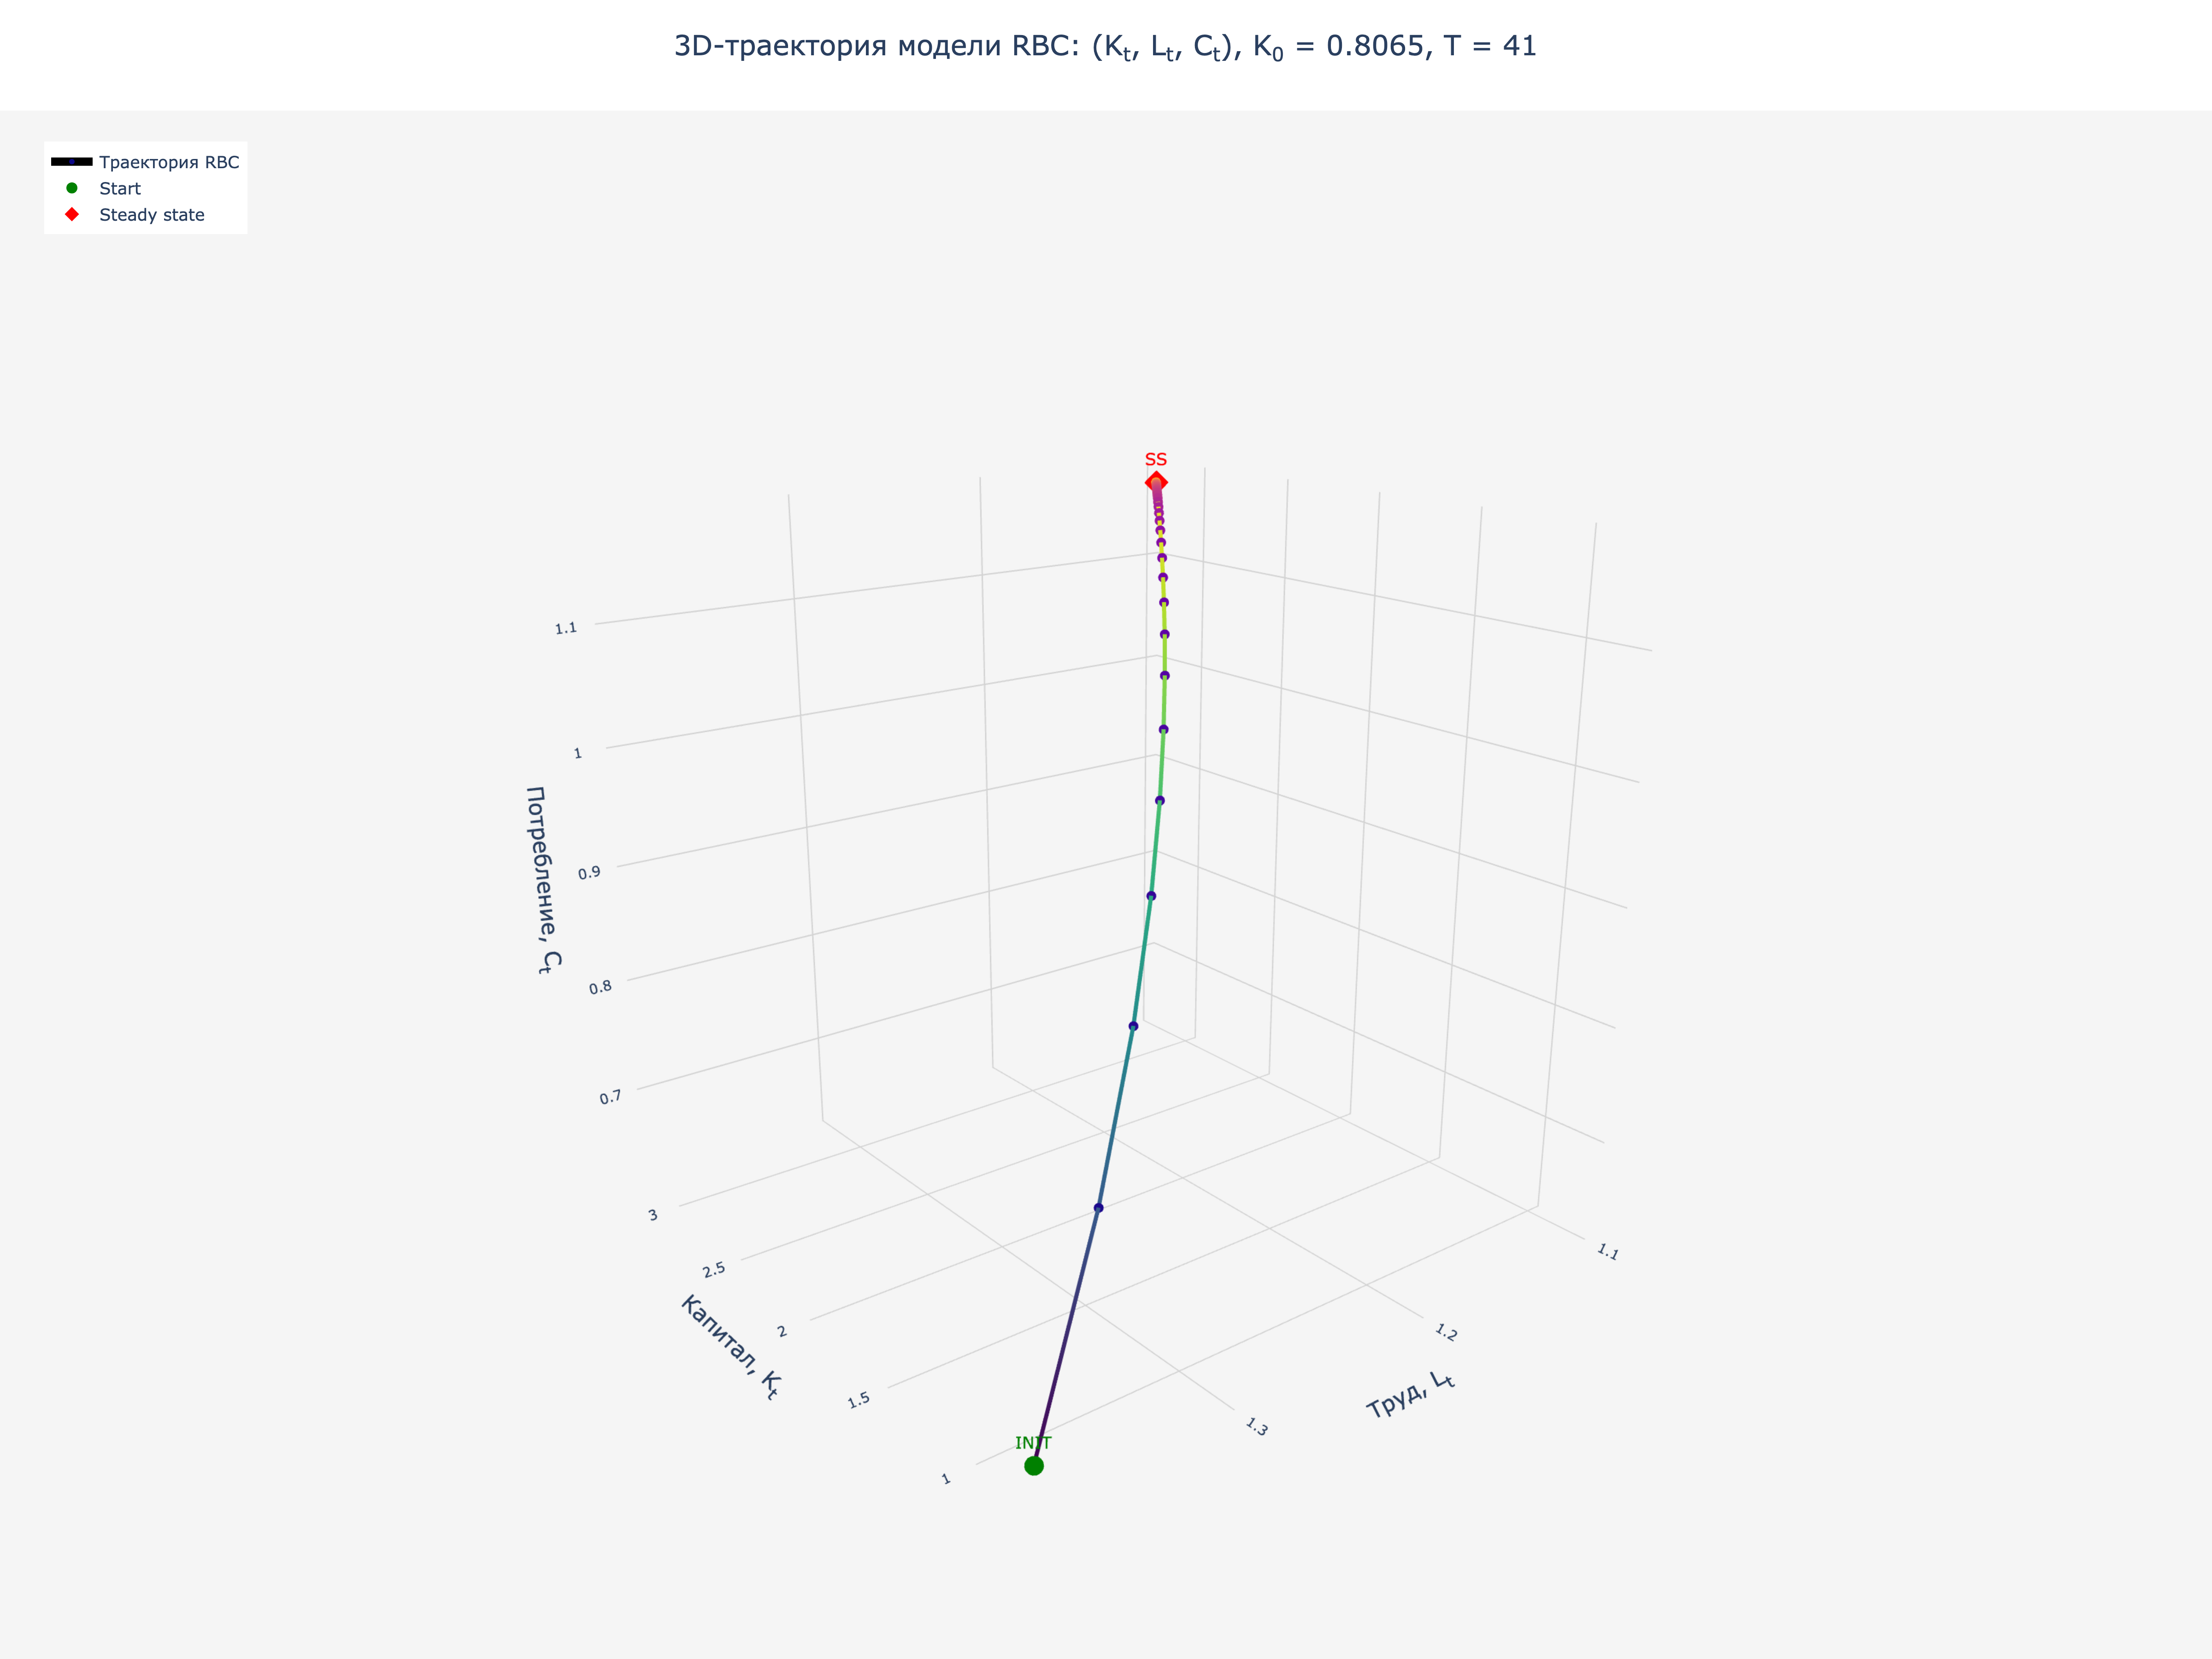
\includegraphics[width=\linewidth,height=0.68\textheight,keepaspectratio]{plots/rbc_trajectory_3d_0.8065.png}
\end{minipage}
\hfill
\begin{minipage}{0.49\textwidth}
    \centering
    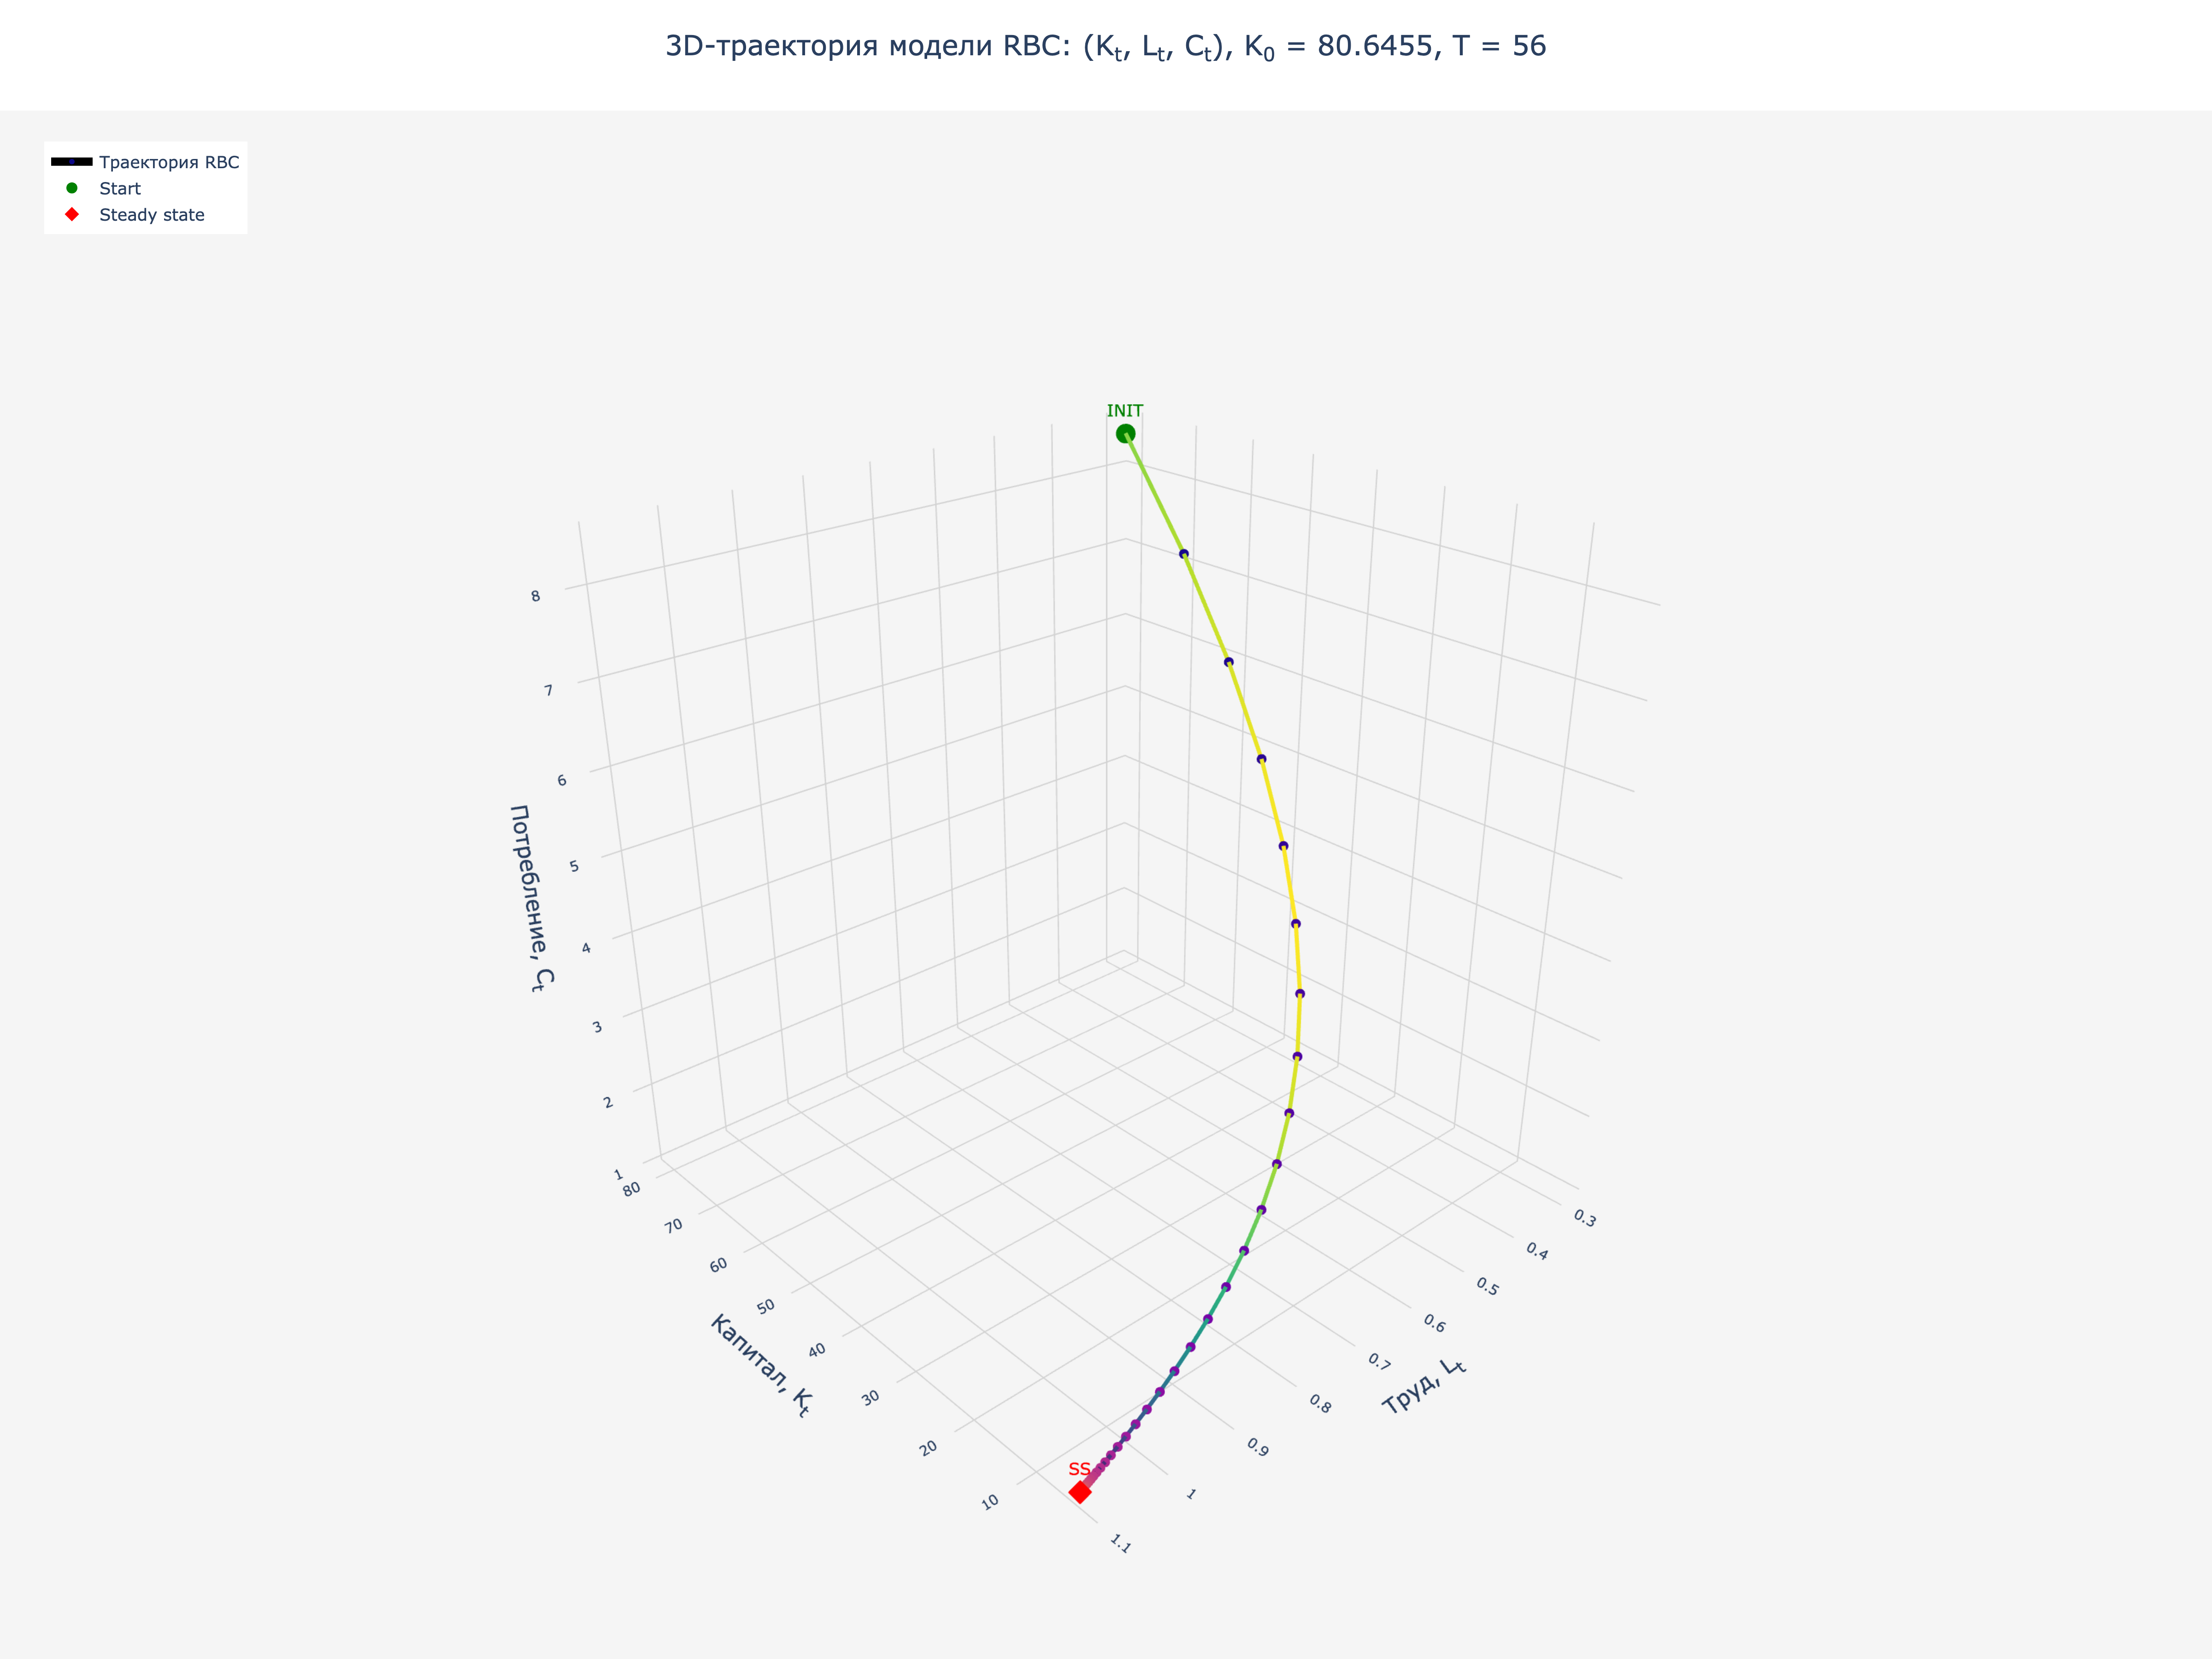
\includegraphics[width=\linewidth,height=0.68\textheight,keepaspectratio]{plots/rbc_trajectory_3d_80.6455.png}
\end{minipage}
\end{frame}

\begin{frame}[fragile]{Необходимые доработки}
\setlstep{0.3cm}{0cm}{0cm}
\begin{itemize}
        \item Реализовать глобальное решение стохастической модели
        \item Провести численные симуляции импульсных откликов
        \item Показать отличия между детерминированным и стохастически SS

\end{itemize}
\end{frame}


\begin{frame}{Конец}
    \centering
    \huge Спасибо за внимание!
\end{frame}


\end{document}
